% !TEX root = 0_main.tex
\chapter{Sequential Garbled Circuits}
Sequential circuits can be used as a very compact circuit description.
In the following section we first describe the concept of sequential circuits (\sect{sec:sqcirc}) using an example and then explain the modifications required to garble/evaluate them.

\section{Sequential Circuits}

\begin{figure}[ht]
    \centering
    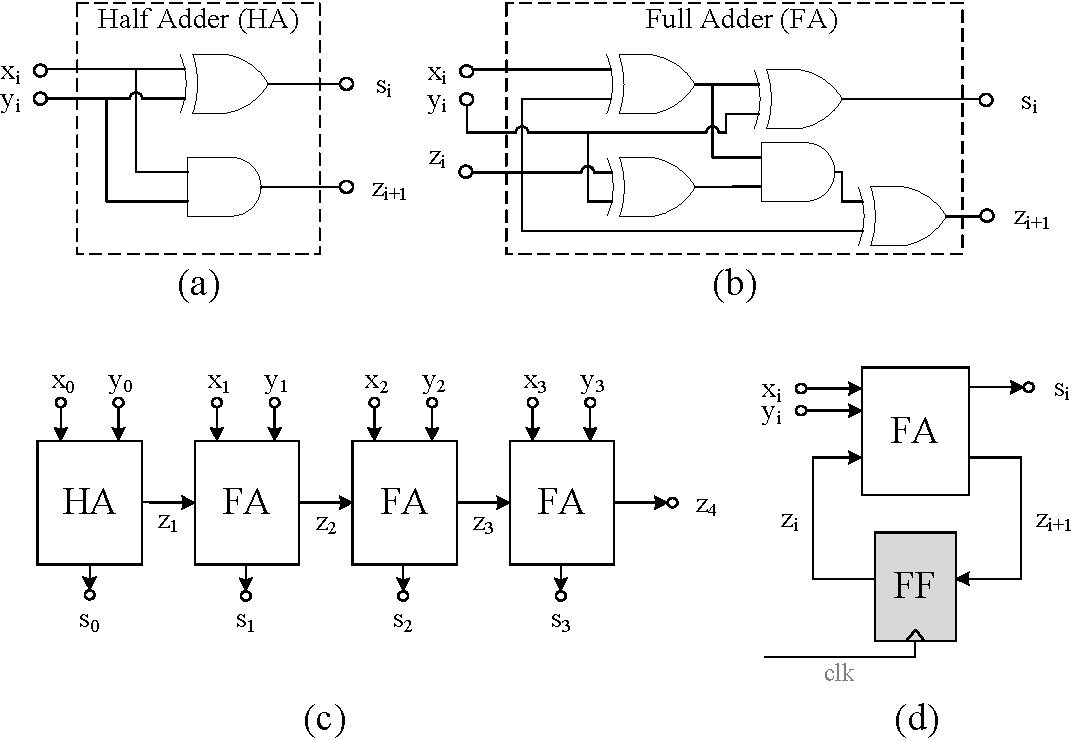
\includegraphics[width=0.7\textwidth]{adder-crop.pdf}
    \caption{Combinational and sequential design of a 4-bit Adder.
  (a) HA circuit.
  (b) FA circuit.
  (c) Combinational 4-bit Adder using 1 HA and 3 FAs.
  (d) Sequential 4-bit Adder using one FA.}\label{fig:combSeq}
\end{figure}

\fig{fig:combSeq} demonstrates an example of a combinational and a sequential implementation for a 4-bit Adder with inputs $x = \overline{x_3x_2x_1x_0}$ and $y = \overline{y_3y_2y_1y_0}$, producing sum $s = \overline{s_3s_2s_1s_0}$.
\fig{fig:combSeq}a and \ref{fig:combSeq}b show the internal combinational circuit of a half Adder (HA) and a full Adder (FA) respectively.
In \fig{fig:combSeq}c a combinational Adder is built by cascading 3 FAs and one HA.
\fig{fig:combSeq}d represents a sequential implementation of a 4-bit Adder which uses one FA and a one bit FF to save the carry bit from the previous cycle.
The circuit should be evaluated in 4 cycles.
At the first cycle the carry bit is $z_0=0$.
Note that, in the combinational circuit we use three FAs and one HA whereas in the sequential circuit, we have to use one FA for 4 sequential cycles.
This asymmetry in the loop of Addition function introduces a very small \emph{overhead} in GC computation and communication time as an HA circuit has fewer gates compared to a FA circuit.

However, the total number of gates for representing the function is reduced approximately by a factor of 4 when using a sequential circuit (one FA for sequential compared with three FA and one HA for combinational).
This helps to limit the memory footprint for garbling and evaluation required for storing circuit description and wire tokens ($k$-bit per wire, see \sect{subsec:preli_GC}).
In a sequential circuit, the number of tokens that need to be stored in memory at any moment is proportional to the number of gates in the circuit.
The wire tokens are simply over-written at each sequential cycle.
Only tokens corresponding to FFs are kept for the next cycle.

Nearly all commercial circuits used in digital hardware are designed in sequential format.
There are multiple reasons for preferring sequential circuit description over combinational including the reduction in complexity, area, power, and cost, as well as natural mapping of finite state machine control functions into a sequential format.
Some of these reasons also provide a rationale for sequential description of a function in GC, including: (i) reduction in size and memory footprint that is achieved by introducing the state elements and feedback loop from output to input; (ii) removing the need to perform costly compile-time/runtime loop unrolling by embracing loops within the sequential feedback loop; (iii) providing a new degree of freedom for folding by the placement of memory elements in the long combinational paths--the placement can be done in accordance with the user's objective.

\begin{figure}[ht]
    \centering
	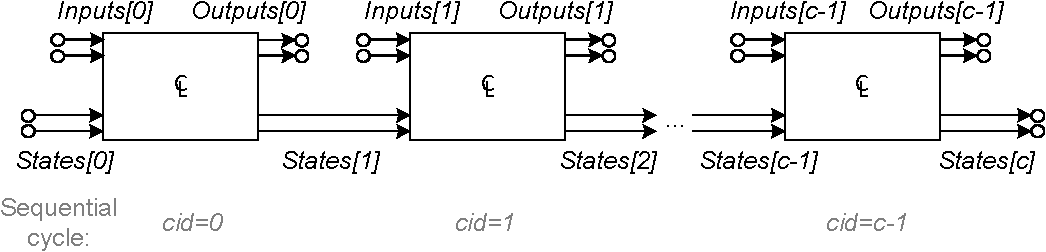
\includegraphics[width=0.8\textwidth]{sequential-open-crop.pdf}
	\caption{Functionally equivalent unrolled sequential circuit corresponding to \fig{fig:sequential}.}
	\label{fig:open-sequential}
\end{figure}

During the evaluation of a sequential circuit, the combinational block is evaluated $c$ times where $c$ is the number of sequential cycles that the circuit operates.
We can visualize this process as the unrolled combinational representation of the sequential circuit as shown in \fig{fig:open-sequential}.
The inputs/outputs of the unrolled circuit are the inputs/outputs of the combinational block in all the cycles.
The present states at each cycle $\textrm{cid}$, where $0 \le \textrm{cid} < c$, are equal to the next states at the previous cycle ($\textrm{cid}-1$).
The present states at $\textrm{cid}=0$ are equal to the input initial value.

During generation and evaluation of the garbled circuit, it must be ensured that the encryption tweaks $T$ (see \sect{subsec:preli_GC}) for each gate is unique because otherwise security is broken \cite[Sect. 3.4]{henecka2013faster}.
In TinyGarble, to ensure the uniqueness property, we set tweak $T$ for each gate to be the concatenation of the cycle index (cid) and the unique gate identifiers (gid) in the combinational part of the sequential circuit, i.e., $T = \textrm{cid} || \textrm{gid}$.
\footnote{An alternative method would be to use a monotonic counter in the circuit generation/evaluation routines which is increased by one for each gate.}
As in previous work, security and correctness of the GC garbling/evaluation follow from the uniqueness of the tweak $T$ and the existing proofs of security and correctness, see \cite{lindell2009proof,bellare2013efficient}.

\section{Synthesis Sequential Circuit}
For synthesis of sequential circuits, the technology library includes memory elements.
These elements can be implemented as FFs which are connected to a clock signal.
Although in conventional ASIC design FFs are typically as costly as four AND gates, in our GC application, FFs do not have any impact on the garbling/evaluation process as they require no cryptographic operations.
Therefore, we set the area of FFs to 0 to show its lack of impact on computation and communication time of garbling/evaluation.
Moreover, we modify our FFs such that they can accept an initial value.
This helps us remove extra MUXs in standard FF design for initialization.


Fortunately, the sequential description helps to overcome most limitations as it generates more compact circuits.
Sequential circuits are radically smaller than combinational ones with the same functionality.
This property allows synthesis tools to perform more effective circuit optimization.
Moreover, the compatibility of our sequential descriptions with standard synthesis tools simplifies the workflow of circuit generation for SFE applications.

\section{Overhead of Sequential Garbled Circuit}
